\documentclass[a4paper]{article}     
\usepackage{amsfonts}
\usepackage{amsmath}
\usepackage{amssymb}
\usepackage{graphicx}


\begin{document}

\noindent \large Auteur: Xander De Blauwer \\
\noindent \large Studierichting: Informatica\\
\noindent \large Oefeningenreeks 5J nr. 2.4\\

\medskip

$\left\{
\begin{array}{l}
x(t) = a\cos^3(t) \\
y(t) = a\sin^3(t) \\
\end{array}
\right.$ \\

$x'(t) = -3a\cos^2(t)\sin(t) $ \\

$y'(t) = 3a\sin^2(t)\cos(t) $ \\

$S = \displaystyle\int_{0}^{2\pi} \sqrt{9a^2\cos^4(t)\sin^2(t) + 9a^2\cos^2(t)\sin^4(t)}dt $ \\

$ = 3a \displaystyle\int_{0}^{2\pi} \sqrt{\cos^2(t)\sin^2(t)(\cos^2(t) + sin^2(t))}dt $ \\

$ = 3a \displaystyle\int_{0}^{2\pi} \cos(t)\sin(t)dt $ \\

$ = 4 \cdot 3a \displaystyle\int_{0}^{\tfrac{\pi}{2}} \cos(t)\sin(t)dt $ \\ 

Stel $x = \sin(t) \Rightarrow dx = \cos(t)dt $ \\

$ = \dfrac{4 \cdot 3}{2}a \left[\sin^2(t)\right]_{0}^{\tfrac{\pi}{2}} $ \\

$ = 6a $ \\




\begin{figure}[h]
\centering
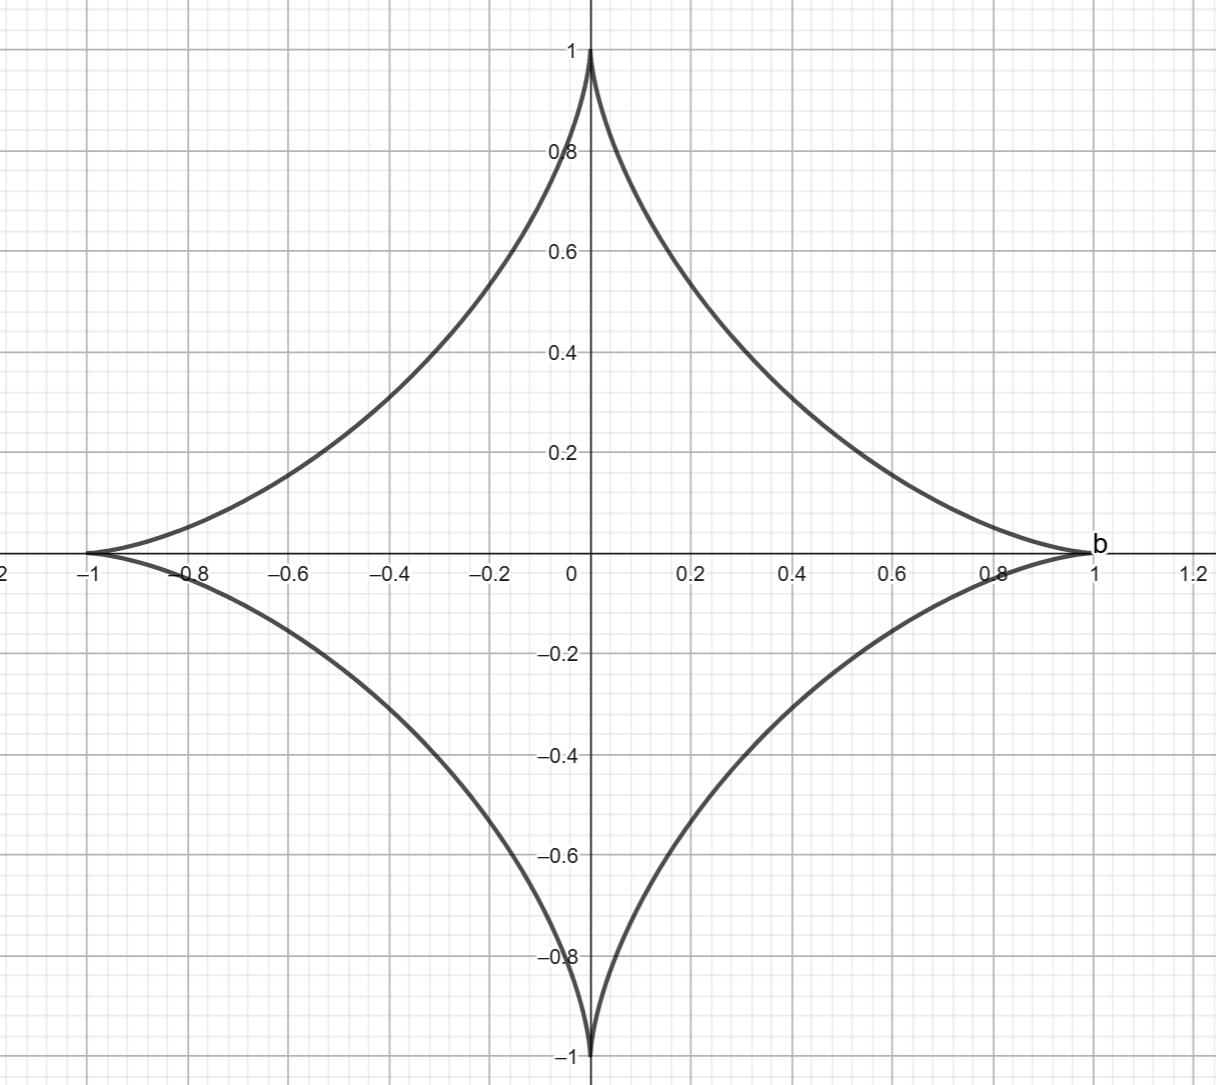
\includegraphics[width=5cm]{5J-2.4-xander.de.blauwer.INF.png}
\end{figure}


\begin{thebibliography}{999}
%\bibitem{a} Referentie
\end{thebibliography}
\end{document} 